\documentclass[]{article}
\usepackage{graphicx} % for pdf, bitmapped graphics files
\begin{document}



\title{Modification of Guidance Law}
\author{Vladimir N. Dobrokhodov}
\date{03/18/2013}
\maketitle

The objective of this new modification is to ``eliminate'' the coordinated turn assumption that is currently used to transform the commanded body rates of the kinematic path following (PF) algorithm into the bank angle command used at the input of the autopilot. Overall goal is to improve the path following performance without over-constraining the flight.

For the sake of simplicity the proposed approach assumes the following structure of an idealized lateral channel, see Figure~\ref{fig:LatAP}. Here we recognize two major contributors to the commanded roll angle. 
 
\begin{figure}[thpb]
      \centering
      \includegraphics[width=95mm]{diagram.png}
      \caption{Simplified diagram of lateral channel}
      \label{fig:LatAP}
   \end{figure}
The first one is based on the coordinated turn assumption and uses a well-known kinematic expression connecting the turn rate $\dot{\psi}_{cmd}$ with the roll angle $\phi_{crd}$. 

\begin{equation}
\label{eq:coordturn}
	\phi_{crd}=arctan( \frac { \dot{\psi}_{cmd} \cdot V_a} {g})	
\end{equation}
The second component is the compensation necessary to account for the non-zero longitudinal ( primarily pitching) motion of airplane if the turn is not coordinated.

Equation~\ref{eq:coordturn} assumes that the aircraft, when turning, is in a steady-state coordinated turn and that the sideslip ($\beta$) and pitch ($\theta$) angles are small. However, if these assumptions do not hold there should be some significant difference in the actual turn rate vs. the desired rate commanded by the PF algorithm.  To calculate the actual turn rate with the roll angle calculated from eq.\ref{eq:coordturn} one can use third Euler attitude kinematic equation

\begin{equation}
\label{eq:psidot}
	\dot{\psi}=\frac {q \cdot sin(\phi_{crd})+ r \cdot cos(\phi_{crd})} {cos(\theta)}	
\end{equation}

Since there is a difference, an additional compensation is needed to generate the adjusted roll command that would make the UAV follow the PF commanded turn rate. Let the error between the turn rates corresponding to the nominal coordinated turn $\dot{\psi}_{cmd}$ and free turning flight with commanded $\phi_{crd}$ be defined as:

\begin{equation}
\label{eq:psierr}
	\dot{\psi}_{err}=\frac { g \cdot tan(\phi_{crd})} {V_a} - \frac {q \cdot sin(\phi_{crd})+ r \cdot cos(\phi_{crd})} {cos(\theta)}	
\end{equation}
This error is the difference that needs to be eliminated when computing the desired bank angle command; as before we utilized the assumption of small angle of attack and side-slip. Next, there might be two approaches to the task of converting this error into the corresponding bank angle adjustement. 

\emph{Approach 1}. Calculate the error $\dot{\psi}_{err}$ as in eq.\ref{eq:psierr} and reuse the coordinated turn relation eq.\ref{eq:coordturn} to calculate the compensating value of additional roll angle, see the details in eq.\ref{eq:approach1} and its Simulink implementation  in Fig.~\ref{fig:Approach1} .

\begin{eqnarray}
\label{eq:approach1}
	\ Input \Rightarrow \dot{\psi}_{cmd}, V_a, g, \theta, q, r  \nonumber \\
	\phi_{crd}=arctan( \frac { \dot{\psi}_{cmd} \cdot V_a} {g}) \nonumber  \\
	\dot{\psi}_{err}=\frac { g \cdot tan(\phi_{crd})} {V_a} - \frac {q \cdot sin(\phi_{crd})+ r \cdot cos(\phi_{crd})} {cos(\theta)} \nonumber \\
	\phi_{err}=arctan( \frac { \dot{\psi}_{err} \cdot V_a} {g}) \nonumber  \\	
	\phi_d=\phi_{crd}+\phi_{err}
\end{eqnarray}

\begin{figure}[thpb]
      \centering
      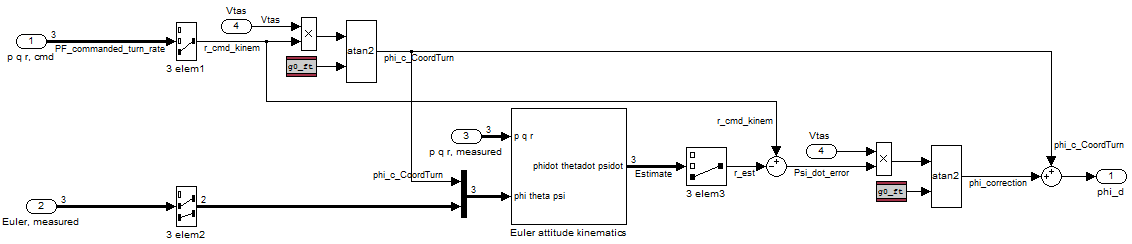
\includegraphics[width=128mm]{approach1.png}
      \caption{Simulink implementation of Approach 1.}
      \label{fig:Approach1}
   \end{figure}

\emph{Approach 2.} If the goal is to eliminate the $\dot{\psi}_{err}$ error in (\ref{eq:psierr}) then one can resolve the equation with respect to the desired roll angle $\phi_d$ assuming that the actual pitching motion is measured and the commanded $\dot{\psi}_{cmd}$ is given by the PF algorithm. See the details in eq.\ref{eq:approach2} and its Simulink implementation  in Fig.~\ref{fig:Approach2}.

\begin{equation}
\label{eq:approach2}
	0=\dot{\psi}_{cmd} - \frac {q \cdot sin(\phi_d)+ r \cdot cos(\phi_d)} {cos(\theta)}~\Rightarrow \phi_d	
\end{equation}

\begin{figure}[thpb]
      \centering
      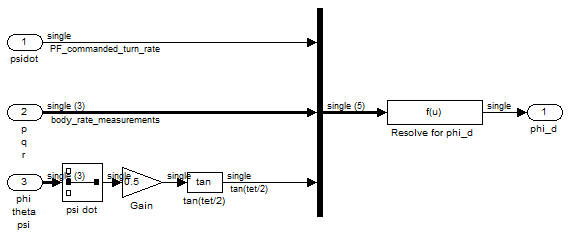
\includegraphics[width=128mm]{approach2.png}
      \caption{Simulink implementation of Approach 2.}
      \label{fig:Approach2}
   \end{figure}

This last equation is resolved analytically in Symbolic Toolbox; see the 2-line script below. There are two solutions to this equation, one them needs to be discarded.

\emph{
$\%\%$ symbolic script that solves 3rd Euler equation with respect to phi angle\\
syms q r tet phid psidot\\
S=solve('psidot-q*sin(phid)/cos(tet)-r*cos(phid)/cos(tet)','phid')\\
}

The following Fig.~\ref{fig:GLAW} illustrates the PF performance of three guidance law algorithms in the same scenario in the presence of a failure. The guidance laws correspond to the (\emph{1-2}) two Approaches presented above and (\emph{3}) the Coordinated turn assumption. All results are obtained with no adaptation enabled. Analysis shows that the results obtained by Approaches \emph{1-2} significantly outperform the Coordinated turn based approach~\emph{3}; it can be also  observed that the Approach 1 and 2 provide very close numerical results that is expected. Not only the PF performance in lateral channel is improved but also the altitude tracking becomes less oscillatory; this is also expected as both approaches account for the pitching motion of the airplane.

\begin{figure}[thpb]
      \centering
      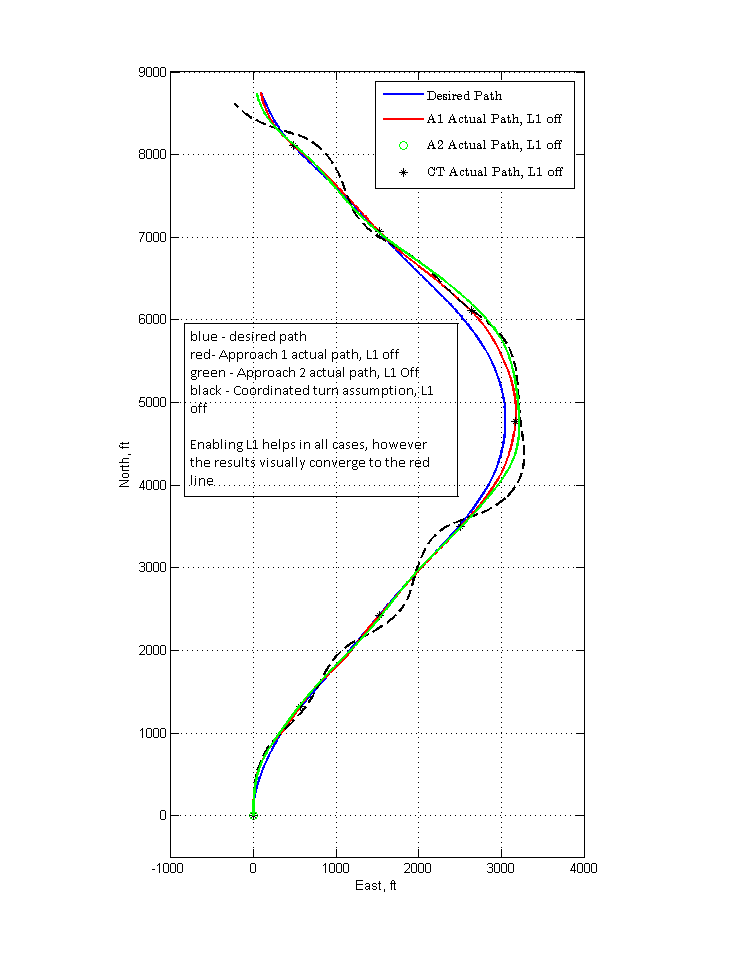
\includegraphics[width=110mm]{NEposition_3Apps.png}
      \caption{Comparison of PF performance of three guidance laws.}
      \label{fig:GLAW}
   \end{figure}

Enabling $L_1$ adaptation improves results of all three approaches. It is worth noting that the contribution of $L_1$  in improving the PF tracking is the ``biggest'' in the case of coordinated turn approach while in the case of newly presented approaches it is minor. 

\end{document}